\documentclass[hyperref={pdfpagelabels=false}]{beamer}
\usepackage{beamerthemesplit}
\usepackage[utf8]{inputenc}
\usepackage[T1]{fontenc}
\usepackage{lmodern}
\usepackage[french]{babel}
\usepackage{graphicx}
\usepackage{tikz}
\usepackage{MnSymbol}

\uselanguage{French}
\languagepath{French}
\usetheme{Green}

\begin{document}
\title{Le logiciel de preuves formelles Coq}
\author{Guillaume Claret}
\date{12 mars 2015}
\maketitle

\section{Démo}
% All template changes are local to this group.
{
  \setbeamertemplate{navigation symbols}{}
  \begin{frame}[plain]
    \frametitle{Démo}
    \begin{tikzpicture}[remember picture,overlay]
      \node[at=(current page.center)] {
        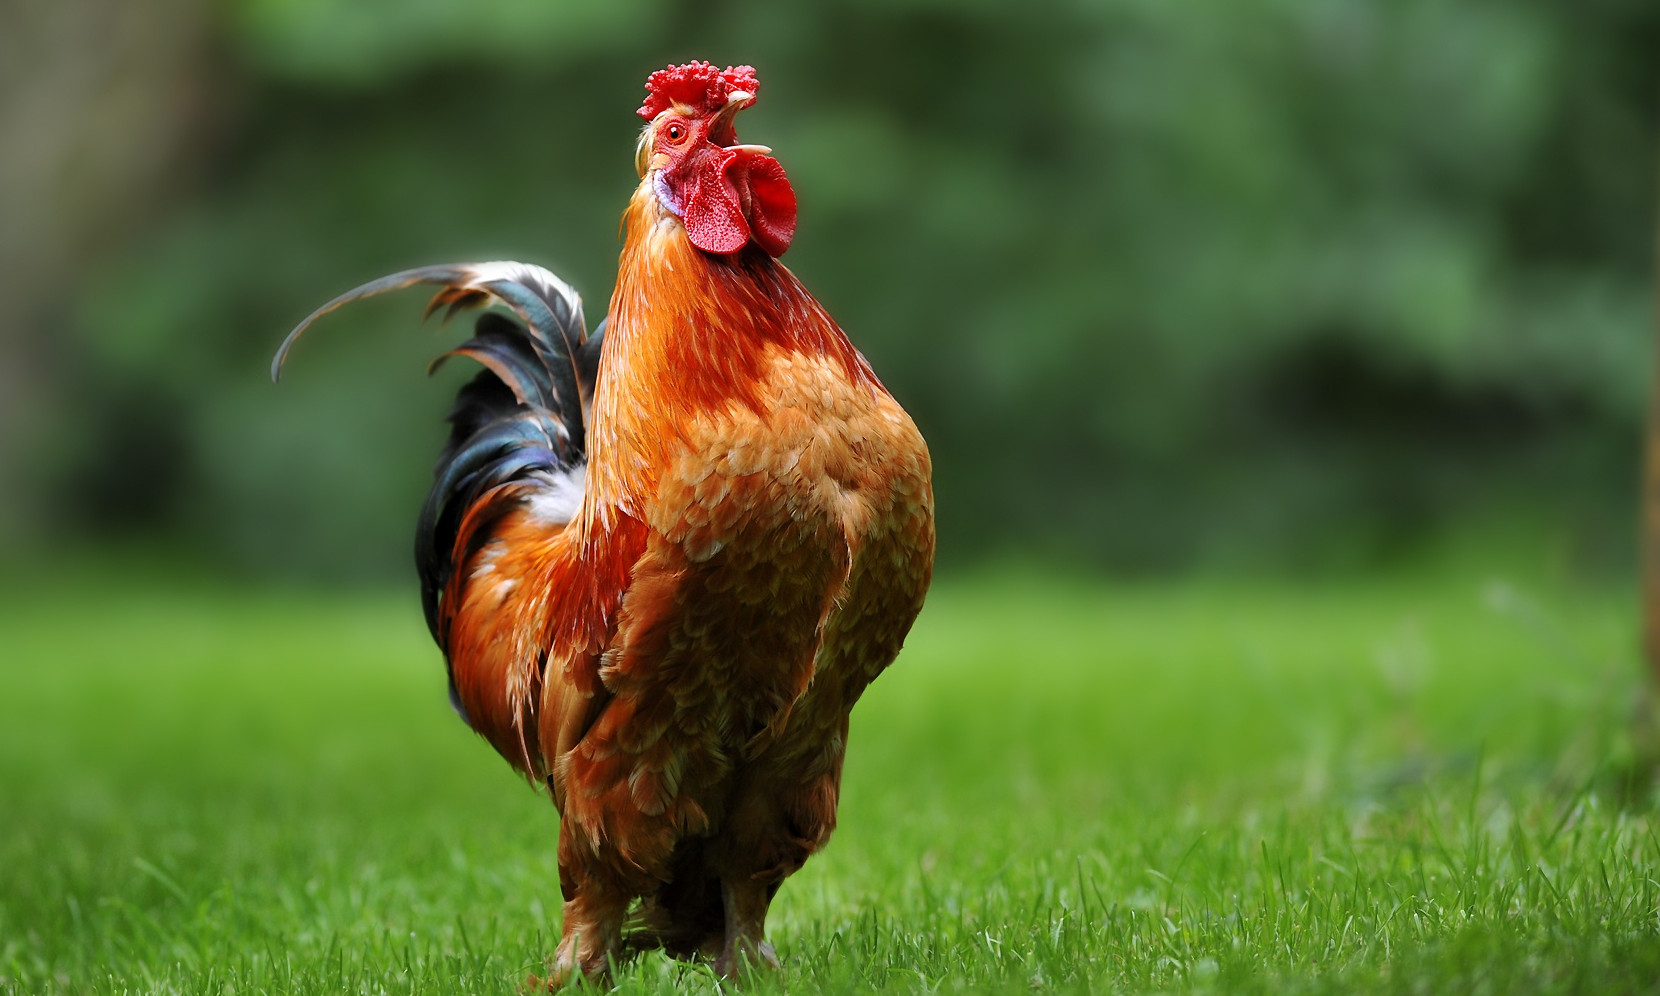
\includegraphics[width=\paperwidth]{images/coq}
      };
    \end{tikzpicture}
  \end{frame}
}

\section{Présentation}
\begin{frame}
  \frametitle{Le logiciel Coq}
  Un language pour:
  \begin{itemize}
    \item énoncer des théorèmes
    \item écrire des preuves formelles
    \item écrire des algorithmes
  \end{itemize}

  Un environnement pour:
  \begin{itemize}
    \item raisonner de façon interactive
    \item organiser / distribuer les développements
  \end{itemize}
\end{frame}

\begin{frame}
  \frametitle{Développements importants}
  \begin{itemize}
    \item théorème des quatre couleurs (Gontier 04)
    \item théorème de Feit -- Thompson (Gontier \& all, 12)
    \item compilateur \textsc{C} CompCert (Xavier Leroy \& all)
    \item bibliothèque \emph{Bedrock} de vérification de programmes bas niveau
  \end{itemize}
\end{frame}

\begin{frame}
  \frametitle{Historique}
  \begin{itemize}
    \item Calcul des Constructions (\textsc{CoC}) par \emph{Thierry Coquand} (85)
    \item implémentation du \textsc{CoC} donnant lieu à \textsc{Coq}
    \item Calculus of Inductive Constructions (\textsc{CiC}) par \emph{Christine Paulin} (91)
  \end{itemize}
\end{frame}

\begin{frame}
  \frametitle{Logique}
  \begin{itemize}
    \item théorie des types plutôt que ensembles
    \item logique intuitionniste et constructive
    \item axiomes du tiers exclu, du choix optionels
  \end{itemize}
\end{frame}

\begin{frame}
  \frametitle{Théorie des types}
  \begin{itemize}
    \item $12 : \mathrm{nat}$
    \item $+ : \mathrm{nat} \rightarrow \mathrm{nat} \rightarrow \mathrm{nat}$
    \item $\mathrm{True} : Prop$
    \item $\forall (A : \mathrm{Prop}),\, A \Rightarrow A : Prop$
    \item $\mathrm{nat} : \mathrm{Set}$
    \item $\mathrm{Set} : \mathrm{Type}$
    \item $\mathrm{Prop} : \mathrm{Type}$
    \item $\mathrm{Type} : \mathrm{Type}$
  \end{itemize}
\end{frame}

\begin{frame}
  \frametitle{Correspondance preuves -- programmes}
  C'est le principal intérêt de la théorie des types. Analogies~:
  \[
    \begin{array}{|c|c|}
      \hline
      \mathrm{Set} & \mathrm{Prop}\\
      A \times B & A \land B\\
      A \cup B & A \lor B\\
      A \rightarrow B & A \Rightarrow B\\
      \forall (x : A),\, B(x) & \forall (x : A),\, B(x)\\
      \mathrm{Programmes} & \mathrm{Preuves}\\
      \mathrm{Types} & \mathrm{Théorèmes}\\
      \hline
    \end{array}
  \]
\end{frame}

\begin{frame}
  \frametitle{Correspondance preuves -- programmes}
  \begin{itemize}
    \item la définition de la logique découle de celle des programmes
    \item il est possible de mélanger preuves et programmes:
      \begin{itemize}
        \item pour prouver des programmes
        \item pour faire des programmes qui prouvent
      \end{itemize}
  \end{itemize}
\end{frame}

\begin{frame}
  \frametitle{Logique intuitionniste}
  \begin{itemize}
    \item tout ce qui est prouvé doit pouvoir être contruit à partir des hypothèses
    \item une preuve de $\exists (x : A),\, P(x)$ permet de calculer $x$
    \item en particulier~: pas de tiers exclu, raisonnement par l'absurde, axiome du choix
    \item tiers exclu et axiome du choix activable en option
  \end{itemize}
\end{frame}

\section{Preuves réflexives}
\begin{frame}
  \frametitle{Preuves réflexives: idée}
    Écrire un programme qui résout une classe de problèmes, en calculant si un problème est vrai ou faux, et le prouver correct.
\end{frame}
\begin{frame}
  \frametitle{Preuves réflexives: exemple}
  Pour un certain type d'équations différentielles, on écrit un programme en \textsc{Coq} qui renvoie \emph{vrai} si il existe une solution positive. On prouve que quand il renvoie \emph{vrai} il existe effectivement une solution positive.

  Alors pour toute équation différentielle de ce type admettant une solution positive, on peut prouver que c'est le cas automatique. Il suffit d'exécuter le programme précédant et d'attendre le résultat.
\end{frame}
\end{document}
